
\chapter{Conforming Finite Element Methods}\label{chap3}

IN\pageoriginale CHAPTER \ref{chap2} WE dealt with the abstract variational
problems and some examples. In all our examples the function space $V$
is infinite dimensional. Our aim is to approximate $V$ by means of
finite dimensional subspaces $V_h$ and study the problem in
$V_h$. Solving the variational problem in $V_h$ will correspond to
solving some system of linear equations. In this Chapter we will study
an error estimate, the construction of $V_h$ and examples of finite
elements. 

\section{Approximate Problem.}\label{chap3:ssec3.1} The
abstract variational problem is:
\begin{equation}\label{chap3:eq3.1}
\text{find } u\varepsilon V \text{ such that } 
a(u, v)=L(v).\quad\text{for all } v\varepsilon V,
\end{equation}
where $a(\cdotp,\cdotp), L(\cdotp), V$ are as in Chapter \ref{chap2}.

Let $V_h$ be a finite dimensional subspace of $V$. Then the
approximate problem corresponding to \eqref{chap3:ssec3.1} is:
\begin{equation}\label{chap3:eq3.2} 
\text{find } u_h\varepsilon V_h \text{ such that } 
a(u_h, v)=L(v)\quad\text{for all } v\varepsilon V_h.
\end{equation}
By the Lax-Milgram Lemma (Chapter \ref{chap2}, Theorem
\ref{chap2:ssec2.1}), \eqref{chap3:eq3.2} has a unique solution.

Let dimension $(V_h)=N(h)$ and let $(w_i)_{i=1,\ldots,N(h)}$ be a
basis of $V_h$. Let 
$$
u_h=\sum\limits_{i=1}^{N(h)}u_iw_i, v_h= 
\sum\limits_{j=1}^{N(h)}v_j
w_j,
$$\pageoriginale
where $u_i, v_j\varepsilon\mathbb{R}$, $1\leq i, j\leq
N(h)$. Substituting these in \eqref{chap3:eq3.2}, we obtain
\begin{equation}\label{chap3:eq3.3}
\sum\limits_{i,j=1}^{N(h)}u_iv_j\; a(w_i, w_j)=
\sum\limits_{j=1}^{N(h)}L(w_j)v_j
\end{equation}
Let 
$$
A^T=(a(w_i, w_j))_{i,j},U=(u_i)_i,\;V=(v_i)_i,b=(L(w_i))_i
$$
Then \eqref{chap3:eq3.3} can be written as 
$$
V^TAU=V^Tb.
$$
This is true for all $V\varepsilon\mathbb{R}^{N(h)}$. Hence 
\begin{equation}\label{chap3:eq3.4}
AU=b.
\end{equation}

If the linear system \eqref{chap3:eq3.4} is solved, then we know the
solution $u_h$ of \eqref{chap3:eq3.2}. This approximation method is
called the Rayleigh-Galerkin method. 

$A$ is positive definite since 
\begin{gather*}
V^TAV=\sum\limits_{i,j=1}^{N(h)} a(w_i, w_j)v_i\; v_j= a\left(
\sum\limits_{i=1}^{N(h)}w_iv_i,\sum\limits_{j=1}^{N(h)}w_jv_j\right)\\
\geq\alpha\parallel\sum\; v_iw_i\parallel^2\quad\text{for all } V
\varepsilon\mathbb{R}^{N(h)}.
\end{gather*}
$A$ is symmetric if the bilinear form $a(\cdotp,\cdotp)$ is symmetric.

From the computational point of view it is desirable to have $A$ as a
sparse matrix, i.e. $A$ has many zero elements. Usually\pageoriginale
$a(\cdotp,\cdotp)$ will be given by an integral and the matrix $A$
will be sparse if the support of the basis functions is ``small''. For
example, if
$$
a(u, v)=\int\limits_\Omega\nabla u.\nabla v\, dx,
$$
then $a(w_i, w_j)=0$ if $\Supp \; w_i\cap\Supp\; w_j=\phi$.

Now we will prove a theorem regarding the error committed when the
approximate solution $u_h$ is taken instead of the exact solution $u$.

\setcounter{THM}{0}
\begin{THM}\label{chap3:THM1}
If $u$ and $u_h$ denote the solutions of \eqref{chap3:eq3.1} and
\eqref{chap3:eq3.2} respectively, then we have 
$$
\parallel u-u_h\parallel_V\leq C\inf\limits_{v_h\varepsilon V_h}
\parallel u-v_h\parallel_V
$$
\end{THM}

\begin{proof}
We have 
\begin{align*}
a(u, v) &= L(v)\quad\text{for all } v\varepsilon V,\\
a(u_h, v) &= L(v)\quad\text{for all } v\varepsilon V_h;
\end{align*}
so
\begin{equation}\label{chap3:eq3.5}
a(u-u_h, v)=0\quad\text{for all } v\varepsilon V_h
\end{equation}

By the $V$-coerciveness of $a(\cdotp,\cdotp)$ we obtain
\begin{align*}
\parallel u-u_h\parallel^2 &\leq 1/\alpha \;a(u-u_h, u-u_h)\\
&= 1/\alpha\;a(u-u_h, u-v+v-u_h), \quad\text{for all } v
\varepsilon V_h\\
&= 1/\alpha\;a(u-u_h, u-v), \quad\text{by \eqref{chap3:eq3.5}}\\
&\leq M/\alpha\; \parallel u-u_h\parallel\;\parallel u-v\parallel
\end{align*}
\end{proof}
This\pageoriginale proves the theorem with $C=M/\alpha$. 

\section{Internal Approximation of $H^1(\Omega)$.}\label{chap3:ssec3.2}
Let $\Omega\subset\mathbb{R}^2$ be a polygonal domain. Let $T_h$ 
be a triangulation of $\Omega$: that is $T_h$ a finite collection 
of triangles such that 
$$
\overline{\Omega}=\bigcup\limits_{K\varepsilon T_h}\overline{K}\quad
\text{and}\quad K\cap K'=\phi\quad\text{for}\quad K, K'\varepsilon
T_h, K\neq K'.
$$

Let $P(K)$ be a function space defined on $K$ such that $P(K)\subset
H^1(K)$. Usually we take $P(K)$ to be the space of polynomials of some
degree. We have 

\begin{THM}\label{chap3:THM2}
If 
$$
V_h=\left\{v_h\varepsilon C^\circ(\Omega):v_h|_K\varepsilon P(K), K
\varepsilon T_h\right\}
$$
where $P(K)\subset H^1(K)$, then $V_h\subset H^1(\Omega)$. 
\end{THM}

\begin{proof}
Let $u\varepsilon V_h$ and $v_i$ be a function defined on $\Omega$
such that $v_i|_K=\dfrac{\partial}{\partial x_i}(u|_K)$. This makes
sense since $u|_K\varepsilon H^1(K)$. Moreover $v_i\varepsilon
L^2(\Omega)$, since $v_i|_K=\cfrac{\partial}{\partial x_i}(u|_K)
\varepsilon L^2(K)$. We will show that $v_i=\dfrac{\partial u}
{\partial x_i}$ in $\mathscr{D}'(\Omega)$.

For any $\phi\varepsilon\mathscr{D}(\Omega)$, we have 
\begin{align*}
\langle v_i,\phi\rangle &= \int\limits_\Omega v_i\phi\,dx= \sum\limits_{K\varepsilon
T_h}\int\limits_K v_i\phi\,dx= \sum\limits_{K\varepsilon T_h}
\int\limits_K\frac{\partial}{\partial x_i}(u|_K)\phi\,dx\\
&= \sum\limits_{K\varepsilon T_h}-\int\limits_K(u|_K)
\frac{\partial\phi}{\partial x_i}\,dx+\int\limits_K(u|_K)\phi\; n_i^K \,
d\Gamma, 
\end{align*}\pageoriginale
where $n_i^K$ is the $i^{th}$ component of the outward drawn normal to
$\partial K$. So
\begin{equation}\label{chap3:eq3.6}
\langle v_i,\phi\rangle=-\int\limits_\Omega u\frac{\partial\phi} {\partial x_i}
\,dx+\sum\limits_{K\varepsilon T_h}\int\limits_{\partial K}(u|_K)\phi
n_i^K \,d\Gamma
\end{equation}

The second term on the right hand side of \eqref{chap3:eq3.6} is zero
since $u$ is continuous in $\Omega$ and if $K_1$ and $K_2$ are two
adjacent triangles then $n_i^{K_1}=-n_i^{K_2}$. Therefore
$$
\langle v_i, \phi\rangle=-\int\limits_\Omega u.\frac{\partial\phi}{\partial x_i}\,dx
=\left\langle\frac{\partial u}{\partial x_i},\phi \right\rangle
$$
which implies
$$
v_i=\frac{\partial u}{\partial x_i}\quad\text{in}\quad\mathscr{D}'
(\Omega). 
$$
Hence $u\varepsilon H^1(\Omega)$. Thus $V_h\subset H^1(\Omega)$. 

We assume that the triangulation $T_h$ is such that if $K_1, K_2
\varepsilon T_h$ are distinct, then either $\overline{K}_1\cap
\overline{K}_2$ is empty or equal to the common edge of the triangles
$K_1$ and $K_2$. By this assumption we eliminate the possibility of
a triangulation as shown in figure.
\begin{figure}[H]
\centering
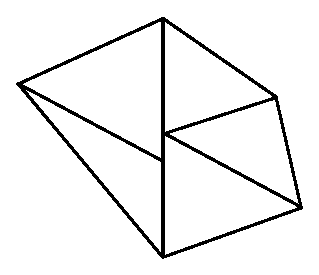
\includegraphics{figure/fig3.1.eps}
\caption{}\label{fig3.1}
\end{figure}

\noindent
{\bf Construction\pageoriginale of $V_h$.} 

Let $\Omega$ be a polygonal domain and $T_h$ be a triangulation of
$\Omega$, where
$$
h=\max\limits_{K\varepsilon T_h}\quad\text{(diameter of $K$)}.
$$
\begin{figure}[H]
\centering
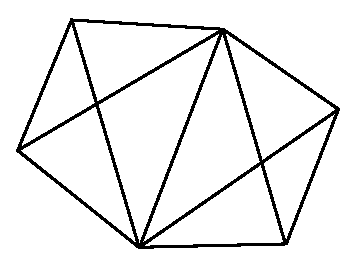
\includegraphics{figure/fig3.2.eps}
\caption{}\label{fig3.2}
\end{figure}

Let

\setcounter{equation}{7}
\begin{equation}\label{chap3:eq3.8}
N(h)=\#\quad\text{nodes of the triangulation},
\end{equation}
\begin{equation}\label{chap3:eq3.9}
\begin{split}
P(K)=P_1(K)=\quad\text{polynomial of degree less than or equal to}\\
 1\quad\text{in}\quad x\quad\text{and}\quad y
\end{split}
\end{equation}
Let
\begin{equation}\label{chap3:eq3.10}
V_h=\{v_h:v_h|_K\varepsilon P_1(K), K\varepsilon T_h\}
\end{equation}

We know that a polynomial of degree $1$ in $x$ and $y$ is uniquely
determined if its values on three non-collinear points are
given. Using this we construct a basis for $V_h$. A function in $V_h$
is uniquely determined if its value at all the nodes of the
triangulation is given. Let the nodes of the triangulation be numbered
$\{1, 2,\ldots,N(h)\}$. Let $W_i\varepsilon V_h$ be
\begin{equation}\label{chap3:eq3.11}
w_i=
\begin{cases}
1\quad\text{at the}\quad i^{th}\quad\text{node},\\
0\quad\text{at other nodes}.
\end{cases}
\end{equation}\pageoriginale
It is easy to see that $w_i$ are linearly independent. If
$v\varepsilon V_h$, then 
\begin{equation}\label{chap3:eq3.12}
v=\sum\limits_{i=1}^{N(h)}v_iw_i
\end{equation}
where $v_i$ the value of $v$ at the $i^{th}$ node. This proves that
$\{w_i\}_{1,\ldots,N(h)}$ is a basis of $V_h$ and dimension of
$V_h=N(h)$.

Moreover, $\Supp w_i\subset\cup\overline{K}$, where the union is taken
over all the triangles whose one of the vertices is the $i^{th}$ node.

Hence if $i^{th}$ node and $j^{th}$ node are not the vertices of a
triangle $K$, for any $K\varepsilon T_h$, then 
$$
\Supp w_i\cap\Supp w_j=\phi.
$$

We will show that $V_h$ given by \eqref{chap3:eq3.10} is contained in
$C^\circ(\overline{\Omega})$. Let $v\varepsilon V_h$ and let $K_1, K_2
\varepsilon T_h$ be adjacent triangles. Let $`\ell'$ be the side
common to both $K_1$ and $K_2$. $v|_{K_1}$ and $V|_{K_2}$ are
polynomials of degree less than or equal to one in $x$ and $y$. Let
$\tilde{v}_1$ and $\tilde{v}_2$ be the extensions of $v|_{K_1}$ and
$v|_{K_2}$ to $\overline{K}_1$ and $\overline{K}_2$
respectively. $\tilde{v}_1|_\ell$ and $\tilde{v}_2|_\ell$ can be
thought of as a polynomial of degree less than or equal to one in a
{\bf single variable} and hence can be determined uniquely if their
values at two distinct points are known. But, by the definition of
$V_h$ in \eqref{chap3:eq3.10},\pageoriginale $\tilde{v}_1|_\ell$ and
$\tilde{v}_2|_\ell$ agree at the common vertices of $K_1$ and
$K_2$. Hence $\tilde{v}_1|_\ell=\tilde{v}_2|_\ell$. This proves that
$v$ is continuous across $K_1$ and $K_2$. Thus $v\varepsilon
C^\circ(\overline{\Omega})$. Hence $V_h\subset
C^\circ(\overline{\Omega})$.

Using the theorem~\ref{chap3:ssec3.2} we conclude that $V_h\subset
H^1(\Omega)$. When we impose certain restrictions on $T_h$, it is
possible to prove that $d(u, V_h)\to 0$ as $h\to 0$ where $d(u, V_h)$
is the distance between the solution $u$ of \eqref{chap3:eq3.1} and
the finite dimensional space $V_h$. The reader can refer to CIARLET
\cite{key9}. Thus $V_h$ ``approximates'' $H^1(\Omega)$. 

The finite element method and the finite difference scheme are the
``same'' when the triangulation is uniform. For elliptic problems the
finite element method gives better results than the finite difference
{\small scheme}.
\end{proof}

\section{Finite Elements of Higher Degree.}\label{chap3:ssec3.3}

\begin{def*}
Let $K$ be a triangle with vertices $(a_i, i=1, 2, 3)$. Let the
coordinates of $a_i$ be $a_{ij},\; j=1, 2$. For any $x\varepsilon
\mathbb{R}$, the \emph{barycentric coordinates} $\lambda_i(x), i=1, 2,
3$, of $x$ are defined to be the unique solution of the linear system 
\begin{equation}\label{chap3:eq3.13}
\begin{split}
\sum\limits_{i=1}^3 \lambda_i\;a_{ij} &= x_j, j=1, 2;\\
\sum\limits_{i=1}^3 \lambda_i &= 1
\end{split}
\end{equation}
\end{def*}

Notice\pageoriginale that the determinant of the coefficient matrix of
the system \eqref{chap3:eq3.13} is twice the area of the triangle
$K$. It is easy to see that the barycentric coordinates of $a_1, a_2,
a_3$ are $(1, 0, 0), \; (0, 1, 0)$ and $(0, 0, 1)$ respectively. The
barycentric coordinate of the centroid $G$ of $K$ is $(1/3,\break 1/3,
1/3)$. 

Using Cramer rule we find from \eqref{chap3:eq3.13} that 
$$
\lambda_1=\dfrac
{\begin{vmatrix}
x_1 & a_{21} & a_{31}\\ 
x_2 & a_{22} & a_{32}\\ 
1 & 1 & 1
\end{vmatrix}}
{\begin{vmatrix}
a_{11} & a_{21} & a_{31}\\ 
a_{12} & a_{22} & a_{32}\\ 
1 & 1 & 1
\end{vmatrix}}
$$
\begin{align*}
\text{i.e.}\hspace{2cm} \lambda_1 &= \dfrac{\text{area of the triangle}
\quad xa_2a_3}{\text{area of the triangle}\quad a_1a_2a_3}\\
\text{Similarly, } \lambda_2 &= \dfrac{\text{area of the triangle}
  \quad a_1xa_3} {\text{area of the triangle}\quad a_1a_2a_3}\\
\lambda_3 &= \dfrac{\text{area of the triangle}\quad a_1a_2x}
{\text{area of the triangle}\quad a_1a_2a_3}
\end{align*}

This geometric interpretation of the barycentric coordinates will be
helpful in specifying the barycentric coordinates of a point. For
example, the equation of the side $a_2a_3$ in barycentric coordinates
is $\lambda_1=0$. 

\begin{def*}
A\pageoriginale {\bf finite element} is a triple $(K, P_K, \sum_K)$, where 
$K$ is a polyhedron, $P_K$ is polynomial space whose dimension is $m$ and
$\sum_K$ is a set of distributions, whose cardinality is $m$. Further
$\sum_K=\{L_i \varepsilon\mathscr{D}';i=1, 2,\ldots,m\}$ is such that
for given $d_i\varepsilon\mathbb{R}$, $1\leq i\leq m$, the equations
$$
L_i(p)=d_i,\; 1\leq i \leq m
$$
have a unique solution $p\varepsilon P_K$.

\noindent The elements $L_i$ are called \emph{degree of freedom of $P$.}
\end{def*}

\setcounter{exam}{0}
\begin{exam}\label{chap3:exm1}
(Finite Element of Degree 1). Let $K=a$ triangle,
\begin{align*}
P_K=P_1(K) &= \text{Polynomials of degree}\leq 1.\\
&= \text{Span}\quad\{1, x, y\}
\end{align*}

$\dim P_K=3$,

$\sum_K=\{\delta_{a_i}:a_i\;\text{vertices},\; i=1, 2, 3\}$,

\noindent where $\delta_{a_i}$ denotes the dirac mass at the point $a_i$. Then
$(K, P_K, \sum_K)$ is a finite element.
\begin{figure}[H]
\centering
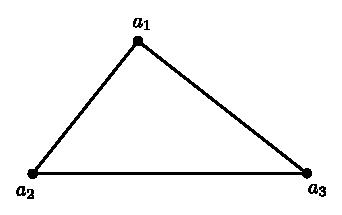
\includegraphics{figure/fig3.3.eps}
\caption{}\label{fig3.3}
\end{figure}

This follows from the fact that $p\varepsilon P_1(K)$ is uniquely
determined if its values at three non collinear points are given.
$$
\delta_{a_i}(\lambda_j)=\lambda_j(a_i)=\delta_{ij}.
$$
Hence\pageoriginale $\lambda_j, j=1, 2, 3$, form a basis for $P_1(K)$
and if $p\varepsilon P_1(K)$ then 
$$
p=\sum\limits_{i=1}^3p(a_i)\lambda_i
$$
\end{exam}

\setcounter{REM}{0}
\begin{REM}\label{chap3:REM1}
In the definition, dimension of $P_K$ is $m$ and we require that the
equations

$L_i(p)=d_i$, $1\leq i \leq m$, for given $d_i\varepsilon\mathbb{R}$
have a solution. So, in examples, to prove existence we have to prove
only uniqueness. To prove the uniqueness it is enough to show that 
$$
L_i(p)=0, 1\leq i\leq m,\quad\text{implies}\quad p\equiv0.
$$
\end{REM}

\begin{REM}\label{chap3:REM2}
If $p_j\varepsilon P_K, 1\leq j\leq m$, are such that 
$$
L_i(p_j)=\delta_{ij}, 1\leq i\leq m, \; 1\leq j\leq m,
$$
then $\{p_j\}$ form a basis for $P_K$ and any $p\varepsilon P_K$ can
be written as 
$$
p=\sum\limits_{i=1}^m L_i(p)P_i.
$$
\end{REM}

\begin{exam}\label{chap3:exm2}
(Finite Element of Degree 2). Let $K=a$ triangle, 
\begin{align*}
P_K &= P_2(K)=\quad\text{Span}\quad \{1, x, y, x^2, xy, y^2\},\\
\sum_K &= \{\delta_{a_i}, 1\leq i\leq 3, \delta_{a_{ij}} :1\leq i<j\leq 3\},
\end{align*}
where $a_i$ denote the vertices of $K$ and $a_{ij}$ denote the mid
point of the side $a_ia_j$.
\begin{figure}[H]
\centering
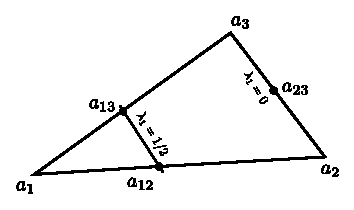
\includegraphics{figure/fig3.4.eps}
\caption{}\label{fig3.4}
\end{figure}


The\pageoriginale equations of the lines $a_3 a_2$ and $a_{13} a_{12}$
are $\lambda_1=0$ and $\lambda_1=1/2$ respectively. Hence the function
$\lambda_1 (\lambda_1-1/2)$ vanishes at the points $a_2, a_3, a_{12},
a_{23}, a_{13}$. The value of $\lambda_1 (\lambda_1-1/2)$ at $a_1$ is
$1/2$. Hence $\lambda_1(2\lambda_1-1)$ takes the value $1$ at $a_1$ and
$0$ at other nodes.

The equations of the lines $a_1 a_3$ and $a_2 a_3$ are $\lambda_2=0$
and $\lambda_1=0$ respectively. Therefore the function
$\lambda_1\lambda_2$ vanishes at $a_1, a_2, a_{13}, a_{23}, a_3$ and
takes the value $1/4$ at $a_{12}$. Thus $4\lambda_1\lambda_2$ is $1$
at $a_{12}$ and zero at the other nodes.

Thus any $p\varepsilon P_2(K)$ can be written in the form 
$$
p=\sum\limits_{i=1}^3p(a_i)\lambda_i(2\lambda_i-1)+\underset{i,
j=1}{\sum\limits_{i<j}^3} 4p(a_{ij})\lambda_i\lambda_j.
$$  
\end{exam}

\begin{exam}\label{chap3:exm3}
(Finite Element of Degree 3). Let $K=a$ triangle, 
$$
P_K=P_3(K)=\quad\text{Span}\quad \{
1,x,y,x^2,xy,y^2,x^3,x^2y,xy^2,y^3\}.
$$

Thus $\dim P_3=10$.
$$
\sum_K=\{ \delta_{a_i}, 1\leq i\leq 3; \; \delta_{a_{iij}} 1\leq i\leq
j\leq 3, \delta_{a_{123}} \}.
$$
where $a_i$ denote the vertices of $K$ and $a_{iij}=\dfrac{2}{3}a_i+
\dfrac{1}{3} a_j$.
\begin{figure}[H]
\centering
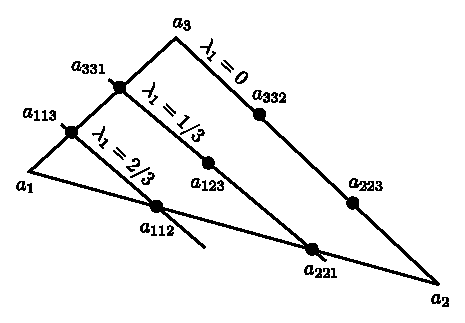
\includegraphics{figure/fig3.5.eps}
\caption{}\label{fig3.5}
\end{figure}


It\pageoriginale is easy to see that 
\begin{align*}
p_i &= 1/2\;\lambda_i(3\lambda_i-1)\; (3\lambda_i-2),\\
p_{iij} &= 9/2\;\lambda_i\lambda_j\; (3\lambda_i-1),\\
p_{123} &= 27\; \lambda_1\lambda_2\lambda_3,
\end{align*}
$1\leq i, j\leq 3$, is a basis of $P_3(K)$.

\noindent Moreover, $p_i$ is $1$ at the node $a_i$ and zero at the
other nodes; $p_{iij}$ is $1$ at the node $a_{iij}$ and vanishes at
the other nodes; $p_{123}$ is zero at all nodes except $a_{123}$ where
its value is $1$.
\end{exam}

\begin{REM}\label{chap3:REM3}
In the above three examples $\sum_K$ contains only Dirac masses and
not derivatives of Dirac masses. All the above three finite elements
are called \emph{Lagrange finite elements}.

Let $\Omega$ be a polygonal domain and let $T_h$ be a triangulation of
$\Omega$, i.e. $\overline{\Omega}=\bigcup\limits_{K\varepsilon T_h}
\overline{K}$. Let $P_K=P_\ell(K)$ consists of polynomials of degree
$\leq\ell$. Let $(K, P_K, \sum_K)$ be a finite element for each $K
\varepsilon T_h$. Let $\sum_h=\bigcup\limits_{K\varepsilon T_h}
\sum_K$ and 
$$
V_h=\{ v_h:v_h|_K\varepsilon P_K, K\varepsilon T_h\}
$$

From\pageoriginale the definition of finite element it follows that a
function in $V_h$ is uniquely determined by the distributions in $\sum_h$.
\end{REM}

\begin{REM}\label{chap3:REM4}
In the example

$\sum_h=\{ \delta_{a_i}:a_i$ is a vertex of a triangle in the
triangulation$\}$.
We proved in Sec. \ref{chap3:ssec3.2} that $V_h\subset
H^1(\Omega)$. In this case we say that the finite element is \emph{conforming}.
\end{REM}

\begin{REM}\label{chap3:REM5}
The $V_h$ so constructed above need not be contained in
$H^1(\Omega)$. If $V_h\nsubset H^1(\Omega)$ we say that the finite
element method is \emph{non-conforming}.

Let $K$ be a triangle, $P_K=P_1(K)$ and
$$
\sum_K=\{ \delta_{a_{ij}}:1\leq i<j\leq 3\}.
$$
Then $(K, P_K, \sum_K)$ will be a finite element, but the space
$V_h\nsubset H^1(\Omega)$.
\begin{figure}[H]
\centering
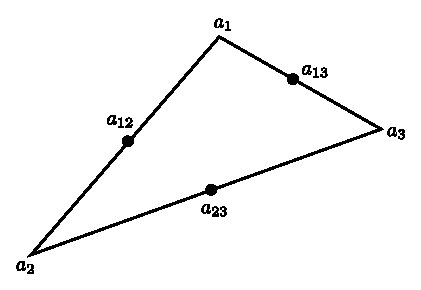
\includegraphics{figure/fig3.6.eps}
\caption{}\label{fig3.6}
\end{figure}
\end{REM}

When\pageoriginale $(K, P_K, \sum_K)$ is as in Example
\ref{chap3:exm2}, we will prove that $V_h\subset
C^\circ(\overline{\Omega})$. This together with theorem
\ref{chap3:ssec3.2} implies $V_h\subset H^1(\Omega)$. Thus the finite
element in Example \ref{chap3:exm2} is conforming. 

To prove that $V_h\subset C^\circ(\overline{\Omega})$, let $K_1$ and
$K_2$ be two adjacent triangles in the triangulation. 
\begin{figure}[H]
\centering
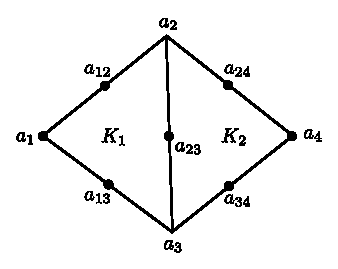
\includegraphics{figure/fig3.7.eps}
\caption{}\label{fig3.7}
\end{figure}


A polynomial of degree 2 in $x$ and $y$ when restricted to a line in
the plane is a polynomial of degree 2 in a single variable and hence
can be determined on the line if the value of the polynomial at three
distinct points on the line are known. Let $v_h\varepsilon V_h$. Let
$\tilde{v}_1$ and $\tilde{v}_2$ be the continuous extension of
$v_h|_{K_1}$ and $v_h|_{K_2}$ to $\overline{K}_1$ and $\overline{K}_2$
respectively; $\tilde{v}_1$ and $\tilde{v}_2$ are polynomials of
degree 2 in one variable along the common side; $\tilde{v}_1$ and
$\tilde{v}_2$ agree at the two common vertices and at the midpoint of
the common side. Hence $\tilde{v}_1=\tilde{v}_2$ on the common
side. This shows $v_h$ is continuous. Hence $V_h\subset
C^\circ(\overline{\Omega})$. 

\setcounter{exercise}{0}
\begin{exercise}\label{chap3:Exr1}
Taking $(K, P_K, \sum_K)$ as in Example \ref{chap3:exm3}, show that
$V_h\subset H^1(\Omega)$.
\end{exercise}

\section{Internal Approximation of $H^2(\Omega)$.}\label{chap3:ssec3.4}
 In\pageoriginale this section we give an
example of a finite element which is such that the associated space
$V_h$ is contained in $H^2(\Omega)$. This finite element can be used
to solve some fourth order problems. We need 

\begin{THM}\label{chap3:THM3}
If $V_h=\{ v_h:v_h|_K\varepsilon P_K\subset H^2(K)$, for all
$K\varepsilon T_h\}$ is contained in $C^1(\overline{\Omega})$ then
$V_h$ is contained in $H^2(\Omega)$. 
\end{THM}

The proof of this theorem is similar to that of theorem
\ref{chap3:THM2} of this section.

\begin{exam}\label{chap3:exm4}
Let $K$ be a triangle 
\begin{align*}
P_K &= P_3(K)=\quad\text{Span}\quad \{ 1,x,y,x^2,xy,y^2,x^3,x^2y,
xy^2, y^3\},\\
\sum_K &= \left\{ \delta_{a_i},\frac{\partial}{\partial x}\delta_{a_i},
\frac{\partial}{\partial y}\delta_{a_i}, \delta_{a_{123}}, 1\leq i\leq 3\right\} 
\end{align*}
where $a_i$ are vertices of $K, a_{123}$ is the centroid of $K$ and 
$$
\dim P_K= \card \sum_K=10.
$$
\begin{figure}[H]
\centering
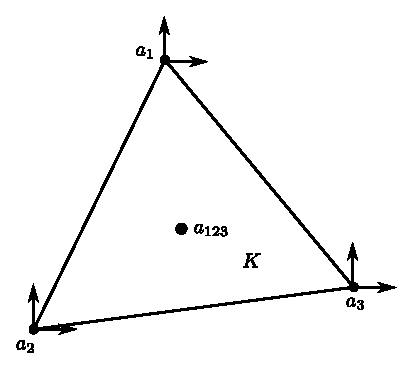
\includegraphics{figure/fig3.8.eps}
\caption{}\label{fig3.8}
\end{figure}


The arrows in the figure denote that the values of the derivatives at
the vertices are given. Using the formula
\begin{align*}
p&=\sum\limits_{i=1}^3\left(-2\lambda_i^3 +3\lambda_i^2 -7\lambda_1\lambda_2\lambda_3\right)
p(a_i)+27\lambda_1\lambda_2\lambda_3 p(a_{123})\\
&\quad+\sum\limits_{1\leq
i< j\leq 3}\lambda_i\lambda_j(2 \lambda_i+\lambda_j -1) Dp(a_i)(a_j -a_i)
\quad \text{ for all }  \quad p\varepsilon P_3
\end{align*}
\pageoriginale

\noindent where
$$
Dp(a_i)=\left( \frac{\partial p}{\partial x}(a_i), \frac{\partial p}
{\partial y}(a_i) \right ).
$$
We obtain that $p\equiv 0$ if 
$$
p(a_i)=p(a_{123})=\frac{\partial p}{\partial x}(a_i)= \frac{\partial
p}{\partial y}(a_i)=0, 1\leq i\leq 3.
$$
Hence $(K, P_K, \sum_K)$ is a finite element.

The corresponding $V_h$ is in $C^\circ(\overline{\Omega})$ but not in
$C^1(\overline{\Omega})$. This shows that $V_h\nsubset
H^2(\Omega)$. Hence this is not a conforming finite element for fourth
order problems.

We now give an example of a finite element with $V_h\subset H^2(\Omega)$.
\end{exam}

\begin{exam}\label{chap3:exm5}
{\bf The Argyris Triangle}. The Argyris triangle has 21 degrees of
freedom. Here the values of the polynomial, its first and second
derivatives are specified at the vertices; the normal derivative is
given at the mid points.

In the figure we denote the derivatives by circles and normal
derivative by a straight lines. 
\begin{figure}[H]
\centering
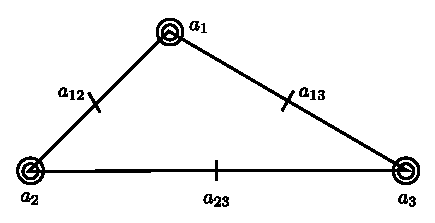
\includegraphics{figure/fig3.9.eps}
\caption{}\label{fig3.9}
\end{figure}\pageoriginale

We take $P_K=P_5=$ Space of polynomials of degree less than or 
\begin{multline*}
\text{equal to} 5.\\
\dim P_K=21;\\
\sum_K=\left\{\delta_{a_i}, \frac{\partial}{\partial x}\delta_{a_i},
\frac{\partial}{\partial y}\delta_{a_i}, \frac{\partial^2} {\partial
x^2}\delta_{a_i},\right.\\
\left.\frac{\partial^2}{\partial x\;\partial y}\delta_{a_i},
\frac{\partial^2}{\partial y^2}\delta_{a_i}, 1\leq i\leq 3,
\frac{\partial}{\partial n}\delta_{a_{ij}}1\leq i<j\leq 3\right\},
\end{multline*}
where $a_i$ denote the vertices of $K, a_{ij}$ the midpoint of the
line joining $a_i$ and $a_j$, and $\partial/\partial n$, the normal
derivative.

Let $p\varepsilon P_K$ be such that $L(p)=0, L\varepsilon\sum_K$ We
will prove that $p= 0$ in $K$. $p$ is a polynomial of degree
5 in one variable along the side $a_1 a_2$. By assumption $p$, and
its first and second derivatives vanish at $a_1$ and $a_2$. Hence
$p=0$ along $a_1 a_2$. Consider $\partial p/\partial n$ along $a_1
a_2$. By assumption $\partial p/\partial n$ vanishes at $a_1 a_2$ and
$a_{12}$. Since the second derivatives of $p$ vanish at $a_1, a_2$ we
have the first derivatives of $\partial p/\partial n$ vanish at $a_1$
and $a_2$; $\partial p/\partial n$ is polynomial of degree 4 in one
variable along $a_1 a_2$. Hence $\partial p/\partial n=0$ along $a_1
a_2$. Since $p=0$ along $a_1 a_2$, $\partial p/\partial\tau =0$ along
$a_1 a_2$, where $\partial/\partial\tau$ denote the tangential
derivative, \ie derivative along $a_1 a_2$. Therefore we have $p$ and
its first\pageoriginale derivatives zero along $a_1 a_2$. 
\begin{figure}[H]
\centering
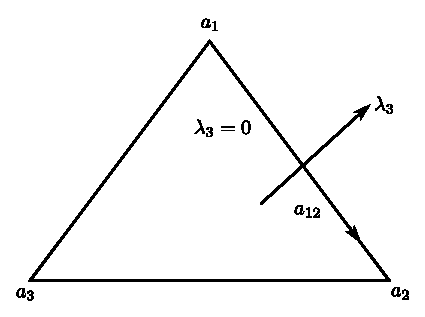
\includegraphics{figure/fig3.10.eps}
\caption{}\label{fig3.10}
\end{figure}


The equation of $a_1 a_2$ is $\lambda_3=0$. Hence we can choose a line
perpendicular to $a_1 a_2$ as the $\lambda_3$ axis. Let $\tau$ denote
the variable along $a_1 a_2$. Changing the coordinates from $(x, y)$
to $(y_3, \tau)$ we can write the polynomial $p$ as 
$$
p=\sum\limits_{i=0}^5 \lambda_3^i q_i(\tau)
$$
where $q_i(\tau)$ is a polynomial in $\tau$ of degree $\leq 5-i$. Now 
$$
\frac{\partial p}{\partial\lambda_3}=\sum\limits_{i=1}^5
i\lambda_3^{i-1} q_i(\tau).
$$
Since $p$ and its first derivatives vanish along $a_1 a_2$ we have 
\begin{align*}
0 &= p(0,\tau)=q_\circ(\tau),\\
0 &= \frac{\partial p}{\partial\lambda_3}(0,\tau)=q_1(\tau) 
\end{align*}
Hence
$$
p=\lambda_3^2\sum\limits_{i=2}^5\lambda_3^{i-2}q_i(\tau).
$$

Thus $\lambda_3^2$ is a factor of $p$. By taking the other sides we
can prove that $\lambda_1^2$ and $\lambda_2^2$ are also factors of
$p$. Thus 
$$
p=c\lambda_1^2\lambda_2^2\lambda_3^2.
$$\pageoriginale
But $\lambda_1^2\lambda_2^2\lambda_3^2$ is a polynomial of degree 6
which does not vanish identically in $K$ and $p$ is a polynomial of
degree 5. Hence $c=0$. Therefore $p\equiv 0$ in $K$. Thus $(K, P_K,
\sum_K)$ is a finite element with 21 degrees of freedom.
\end{exam}

\begin{THM}\label{chap3:THM4}
If $V_h$ is the space associated with the Argyris finite element, then
$V_h\subset C^1(\overline{\Omega})$.
\end{THM}

\begin{proof}
Let $K_1, K_2$ be two adjacent finite elements in the
triangulation. Let $v\varepsilon V_h$ and let $p_1=v|_{K_1}$,
$p_2=v|_{K_2}$. We denote the continuous extensions of $p_1$ and $p_2$
to $\overline{K}_1$ and $\overline{K}_2$ also by $p_1$ and $p_2$. We
have to show that 
$$
p_1=p_2, Dp_1=Dp_2
$$
along the common side $Q$ of $K_1$ and $K_2$. 
\begin{figure}[H]
\centering
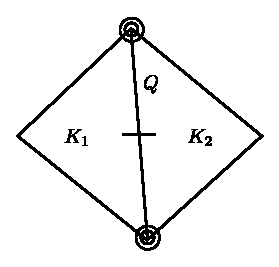
\includegraphics{figure/fig3.11.eps}
\caption{}\label{fig3.11}
\end{figure}

Since $v\varepsilon V_h, p_1, p_2$ their first and second derivatives
agree at the two common vertices of $K_1$ and $K_2$. $p_1$ and $p_2$
are\pageoriginale polynomials of degree 5 in one variable along the
common side $Q$. Hence, along $Q$, 
\begin{equation}\label{chap3:eq3.14}
p_1=p_2.
\end{equation}
Therefore 
\begin{equation}\label{chap3:eq3.15}
\frac{\partial p_1}{\partial\tau}=\frac{\partial p_2}{\partial\tau}
\quad\text{along}\quad Q.
\end{equation}

The normal derivatives $\dfrac{\partial p_1}{\partial n}$ and
$\dfrac{\partial p_2}{\partial n}$ are polynomials of degree 4 in one
variable along $Q$. Since $v\varepsilon V_h$, $\dfrac{\partial p_1}
{\partial n}=\dfrac{\partial p_2}{\partial n}$ at the two common
vertices and at the midpoint of the common side $Q$. Moreover, the
first derivatives of $\dfrac{\partial p_1}{\partial n}$ and
$\dfrac{\partial p_2}{\partial n}$ coincide at the common
vertices. Hence 
\begin{equation}\label{chap3:eq3.16}
\frac{\partial p_1}{\partial n}=\frac{\partial p_2}{\partial n}
\quad\text{along}\quad Q.
\end{equation}
Equations \eqref{chap3:eq3.14} - \eqref{chap3:eq3.16} show that 
$$
p_1=p_2, Dp_1=Dp_2\quad\text{along}\quad Q.
$$
\end{proof}

This proves that $v$ and its first derivative are continuous across
$Q$. Therefore $v\varepsilon C^1(\overline{\Omega})$. Hence
$V_h\subset C^1(\overline{\Omega})$.

Theorems \ref{chap3:ssec3.3} and \ref{chap3:ssec3.4} imply that
$V_h\subset H^2(\Omega)$. For other examples of finite element, the
reader can refer to CIARLET \cite{key9}.

 
